\documentclass[12pt]{article}
\usepackage{geometry}
\geometry{a4paper, total={170mm, 250mm}}
\title{\textbf{Homework 6}}
\author{Maedeh Karkhane Yousefi}
\usepackage{float}
\usepackage{graphicx}
\usepackage{amsmath}
\usepackage{amssymb}
\usepackage{subcaption}
\usepackage{hyperref}
\hypersetup{
    colorlinks=true,
    linkcolor=blue,
    filecolor=magenta,      
    urlcolor=cyan,
    }
\begin{document}
\maketitle
\part*{1. Exercise 6.3: Central Limit Theorem}
\paragraph*{} Knowing that the program's random generator gives a uniform distribution to us, we used this property to sum specific number of random numbers for 10000 samples.
\begin{figure}[H]
	\centering
	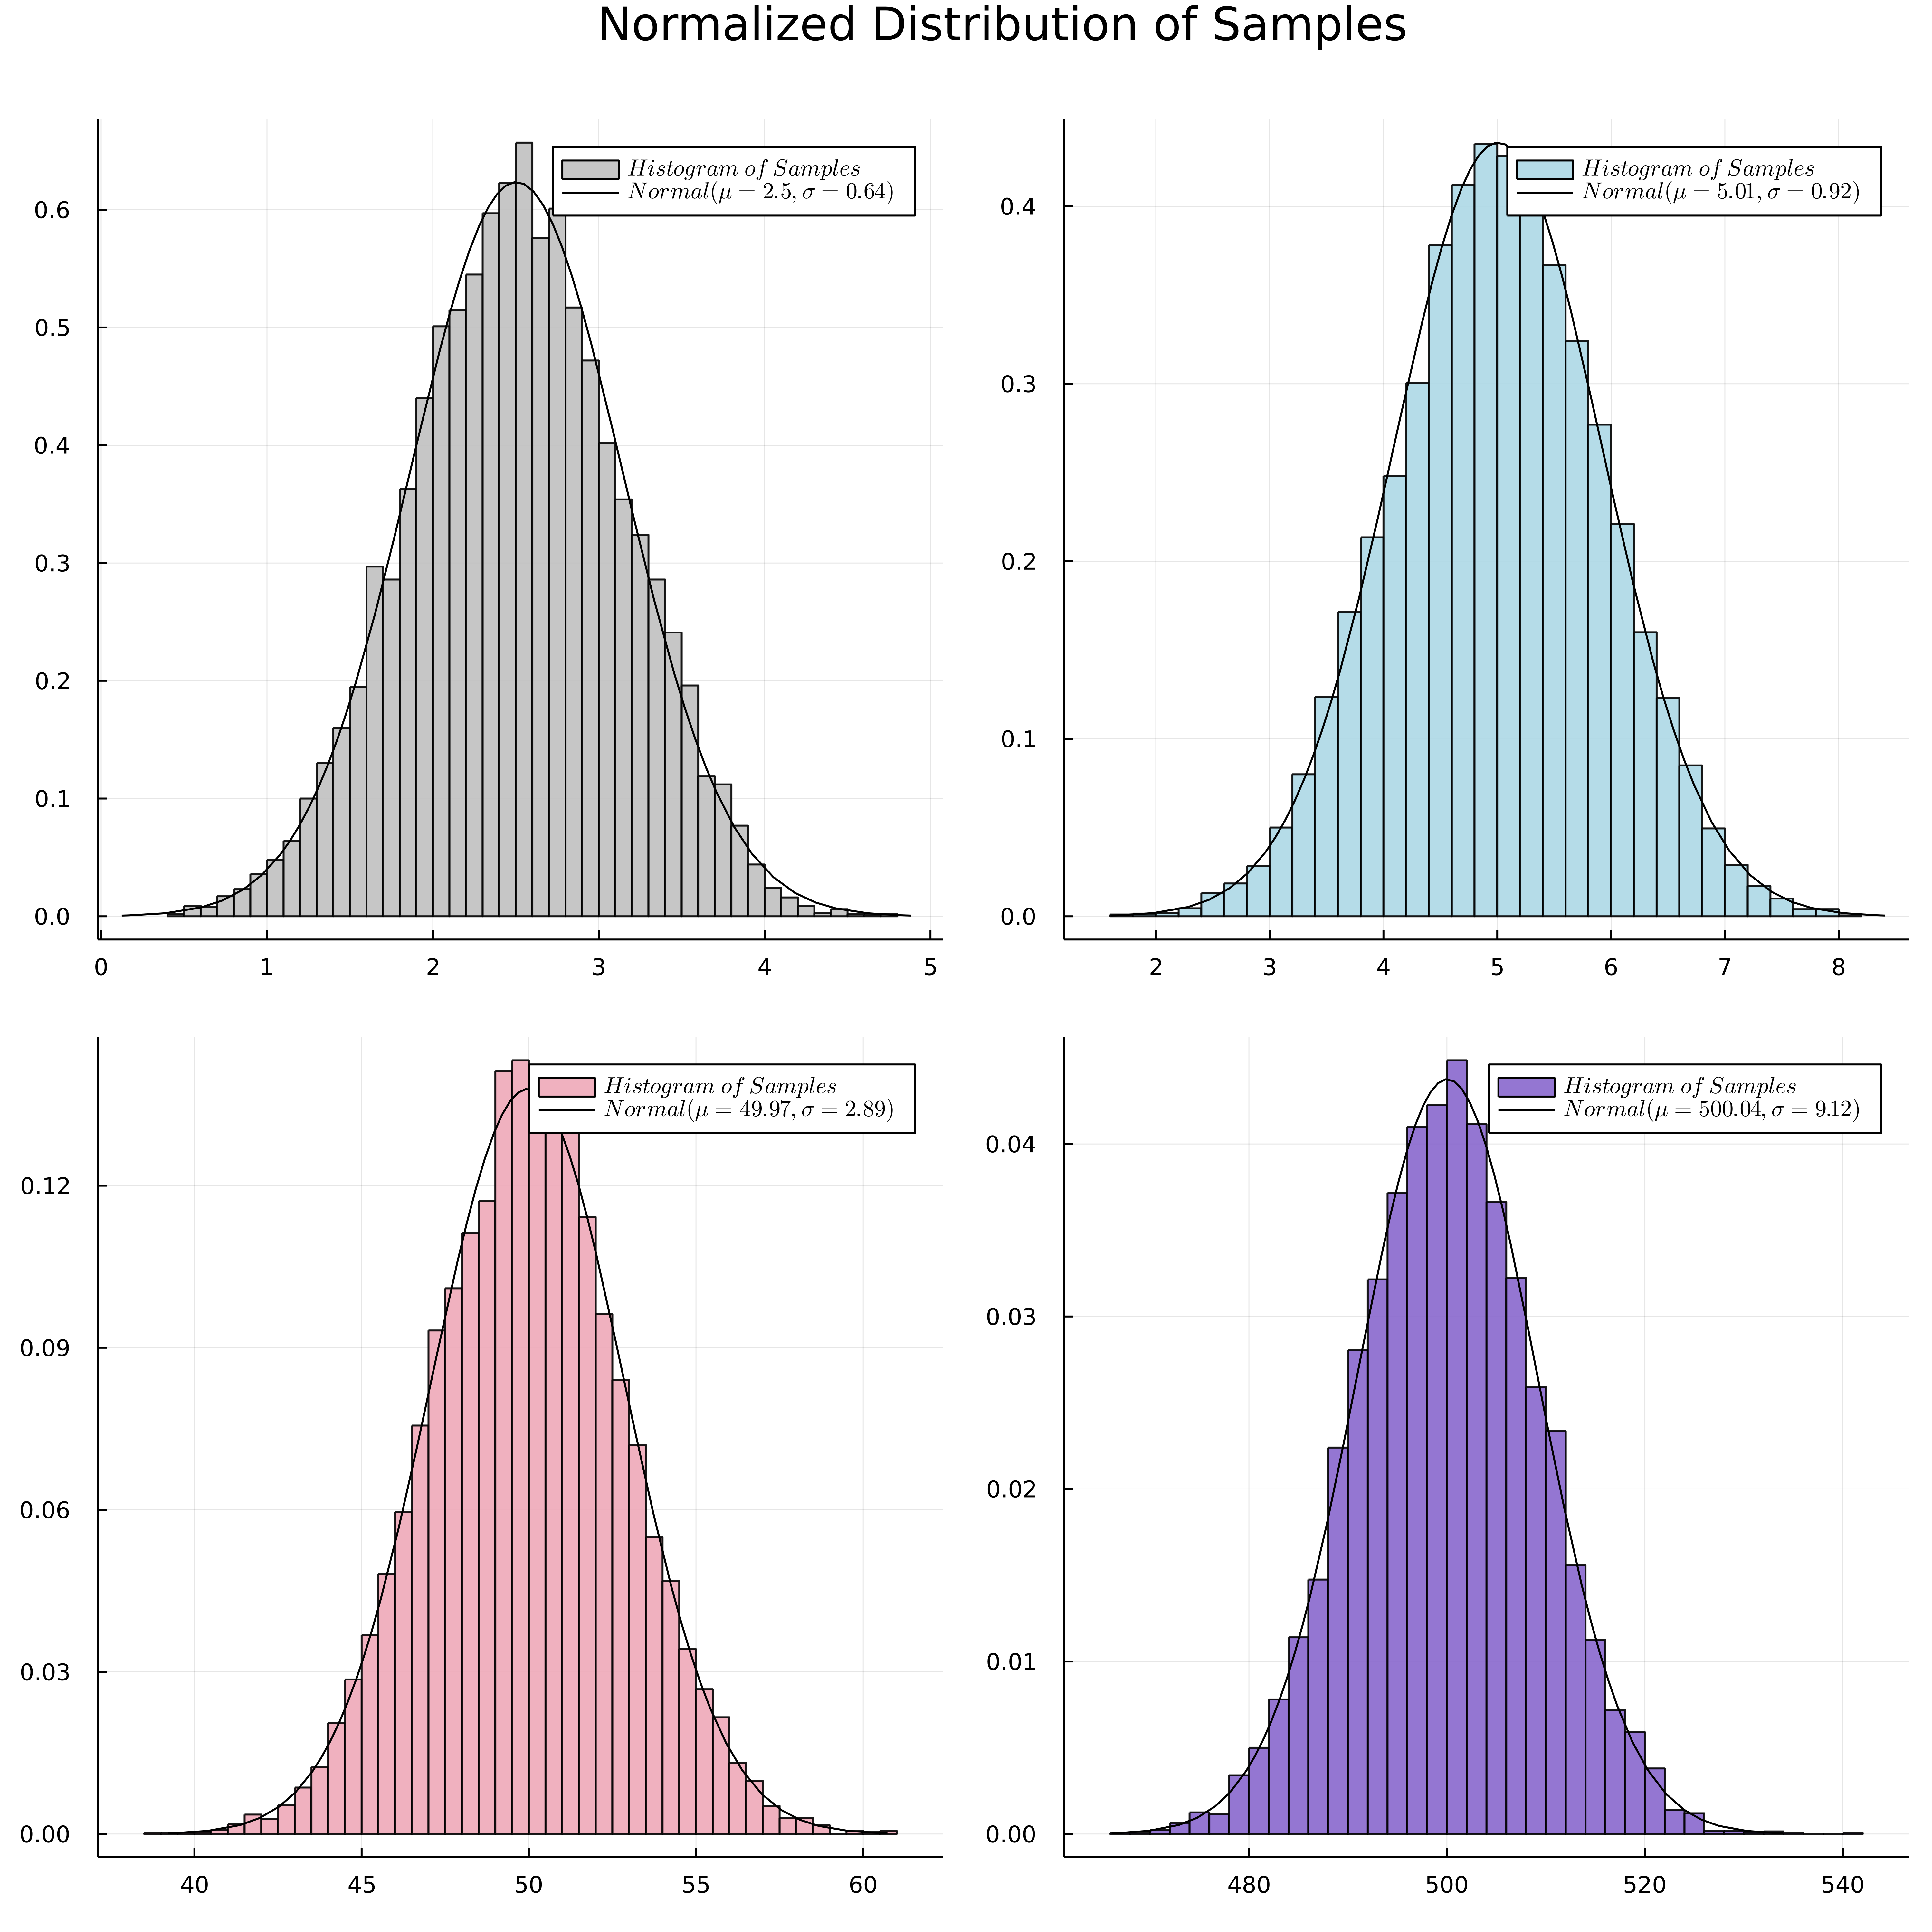
\includegraphics[width=\textwidth]{N_Distribution1.png}
	\label{fig:mesh1}
	\caption{Central Limit Theorem for lengths: 5, 10, 100, 1000 for 10000 samples each. }
\end{figure}
\part*{2. Exercise 6.4: Transformation Matrix}
\begin{gather*}
\int_{a}^{b} \frac{1}{2 \pi \sigma^{2}} \rho \exp \left(-\frac{\rho^{2}}{2 \sigma^{2}}\right) d \rho d \theta\\
f(\rho)=\int_{0}^{\rho} \frac{1}{\sigma^{2}} \exp \left(-\frac{\rho^{\prime 2}}{2 \sigma^{2}}\right) d \rho^{\prime}=x=1-\exp \left(-\frac{\rho^{2}}{2 \sigma^{2}}\right)\\
\rho=\sqrt{-2 \sigma^{2} \ln (1-x)}\\
f(\theta)=\int_{0}^{\theta} \frac{1}{2 \pi} d \theta^{\prime}=x^{\prime}=\frac{\theta}{2 \pi}\\
\theta=2 \pi x^{\prime}\\
y 1=\rho \cos \theta \quad, \quad y 2=\rho \sin \theta
\end{gather*} 
\paragraph*{} With these results, I used an array of randomly generated numbers from the program's uniform distribution algorithm as input and considered N/2 of these elements as x1 and others as x2, and put into these equations. 
\begin{figure}[H]
	\centering
	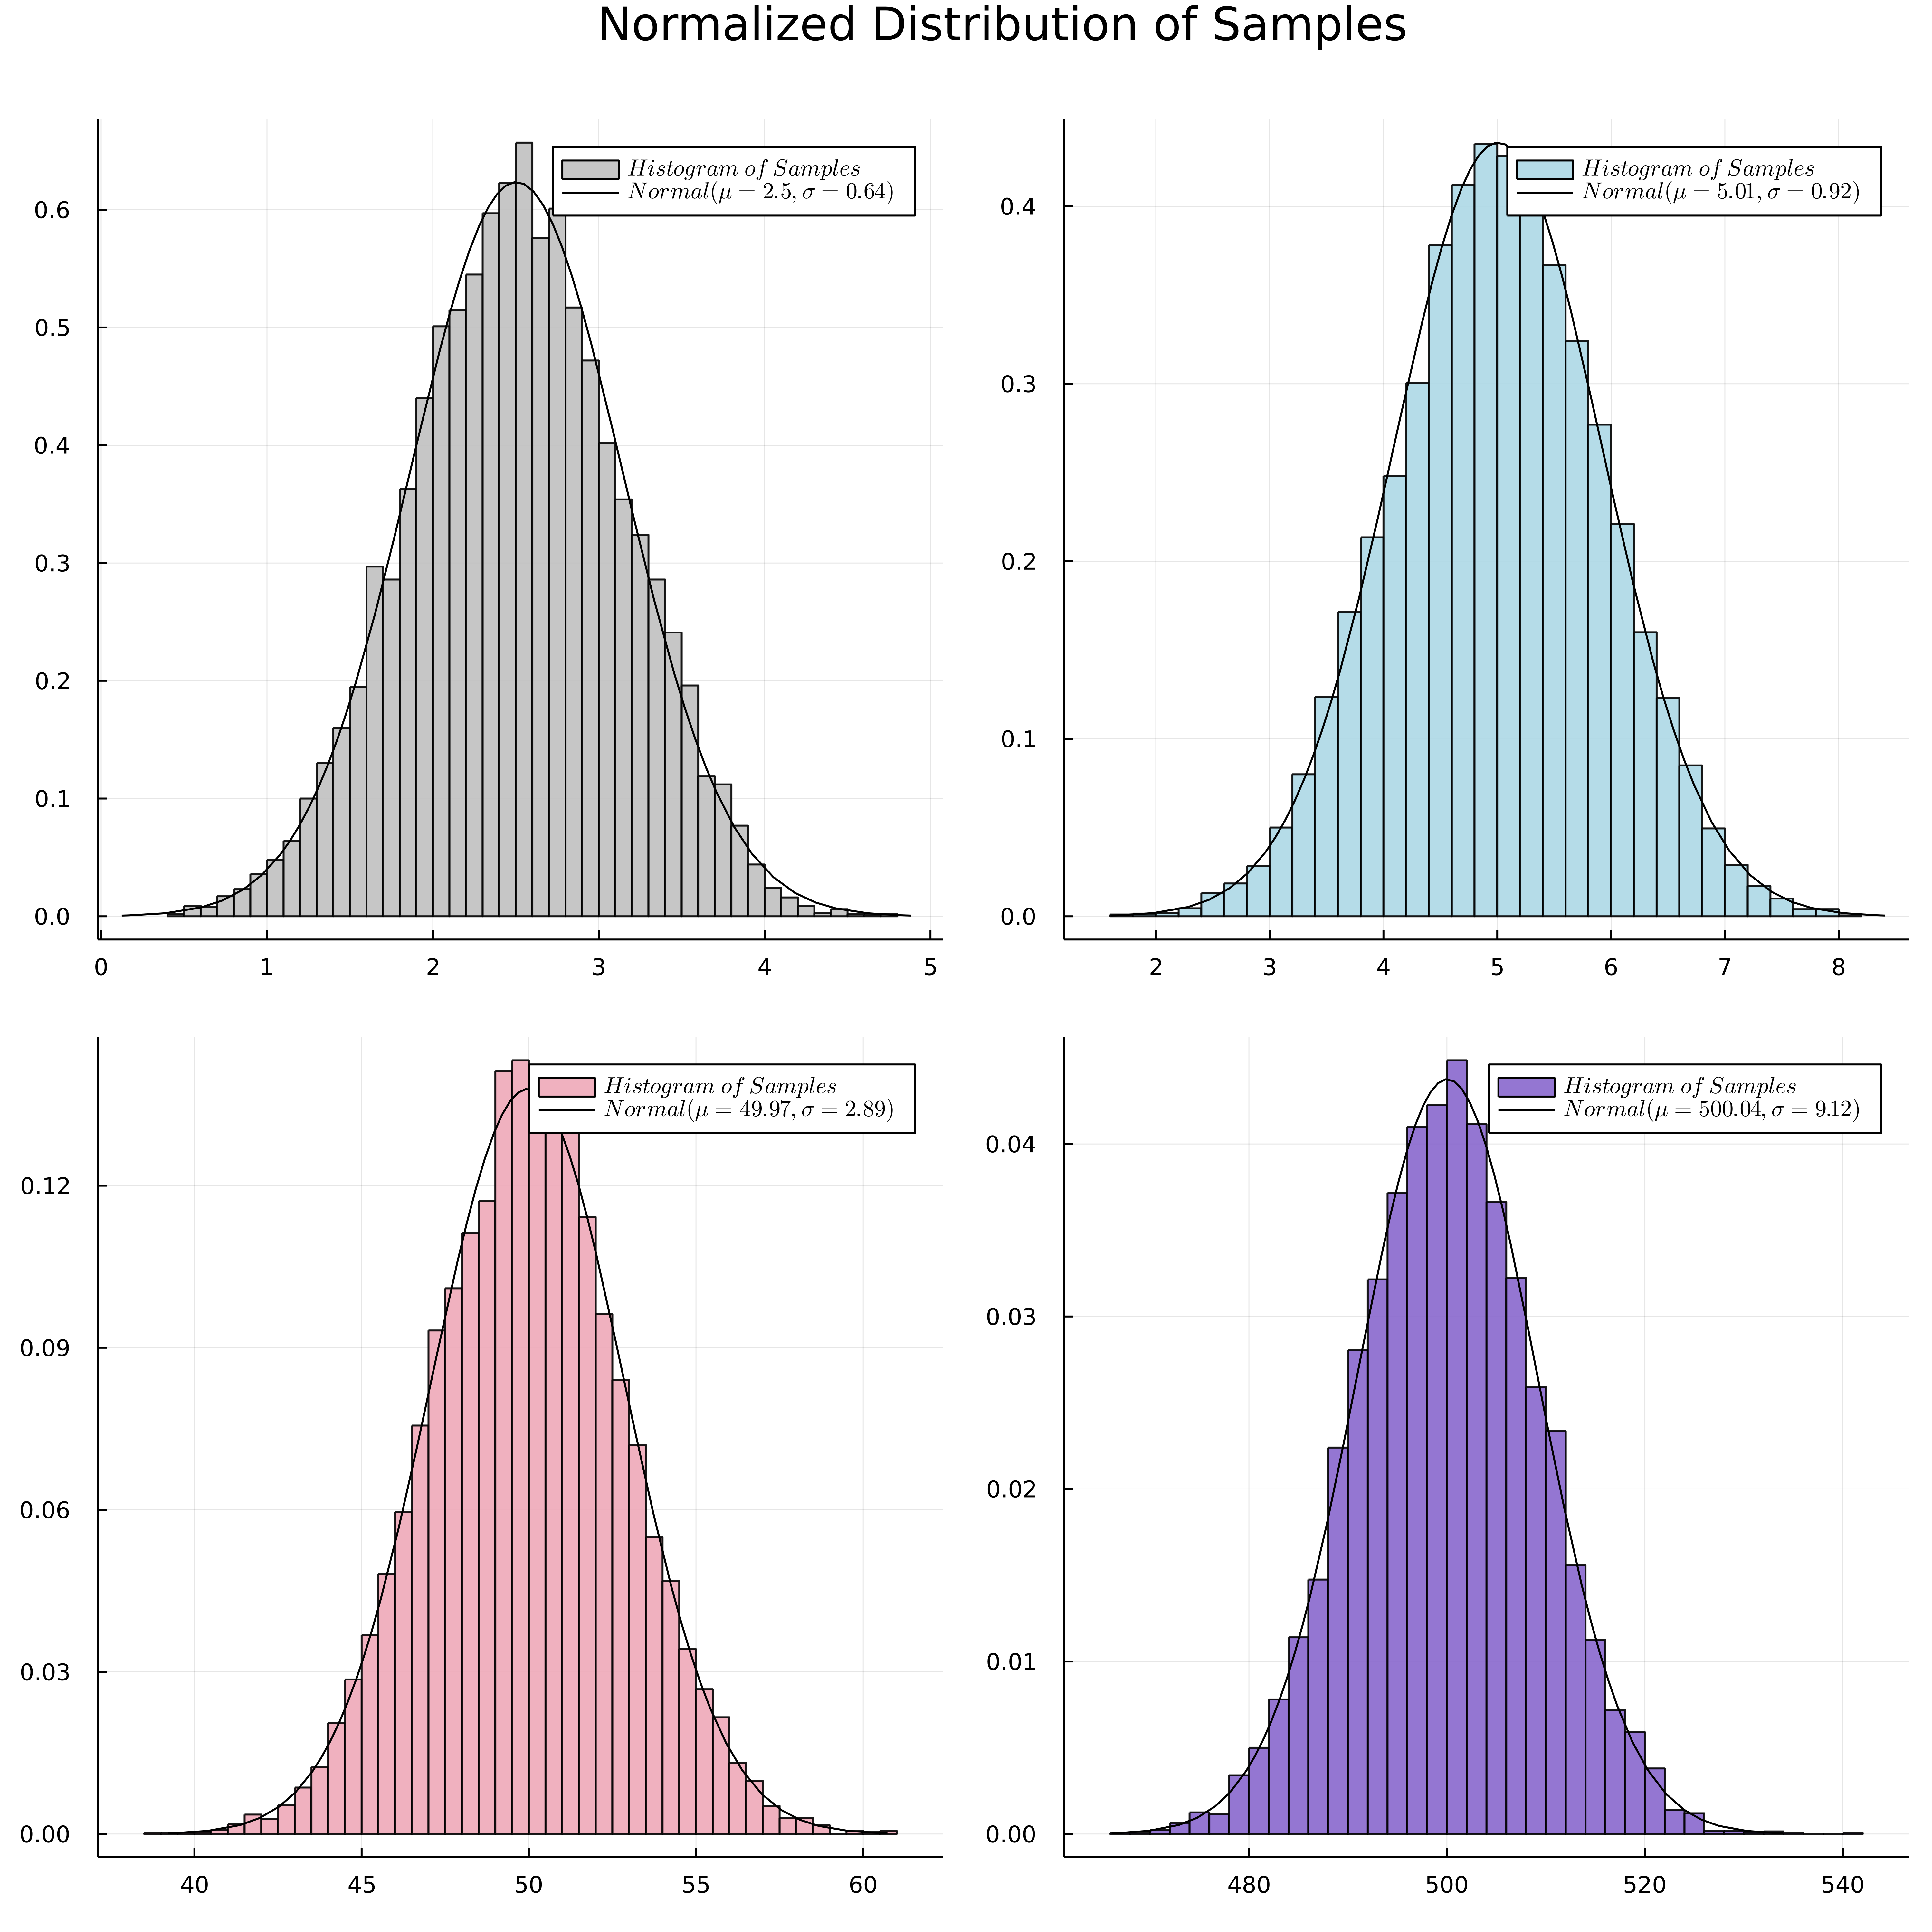
\includegraphics[width=\textwidth]{N_Distribution.png}
	\label{fig:mesh2}
	\caption{Random numbers' distribution using the Box–Muller transform getting use of the program's own uniform distribution random generator. $\sigma$=[1, 2, 3, 4, 5] , Sample Number=1000000}
\end{figure}
    \textbf{use \href{https://github.com/narges8k/computational_physics/tree/main/chapter6}{this link} to check the saved data. }
\end{document}